\documentclass[aspectratio=169, 11pt]{beamer}

% --- Packages ---
\usepackage[utf8]{inputenc}
\usepackage[T1]{fontenc}
\usepackage{lmodern}
\usepackage{graphicx}
\usepackage{booktabs}
\usepackage{amsmath, amssymb}
\usepackage{xcolor}
\usepackage{qrcode}

\usepackage{hyperref}
\usepackage[numbers]{natbib}
\bibliographystyle{model3-num-names}
\renewcommand\UrlFont{\color{blue}\rmfamily}

%% BIBLIOGRAPHY
% Remove "doi:" from DOIs
\providecommand{\DOIprefix}{}
\renewcommand{\DOIprefix}{}

% --- Theme & UDE Color Palette ---
\usetheme{Madrid}
\usecolortheme{default}

\definecolor{udeBlue}{RGB}{0, 76, 147}      % University of Duisburg-Essen Blue
\definecolor{udeLight}{RGB}{230, 238, 246}  % Soft tint for blocks
\definecolor{accentRed}{RGB}{180, 30, 30}   % Highlight color

\setbeamercolor{palette primary}{bg=udeBlue, fg=white}
\setbeamercolor{palette secondary}{bg=udeBlue!85!black, fg=white}
\setbeamercolor{palette tertiary}{bg=udeBlue!70!black, fg=white}
\setbeamercolor{structure}{fg=udeBlue}
\setbeamercolor{frametitle}{bg=udeLight, fg=udeBlue}
\setbeamercolor{block title}{bg=udeBlue, fg=white}
\setbeamercolor{block body}{bg=udeLight!60, fg=black}

% Remove default navigation symbols for a cleaner look
\setbeamertemplate{navigation symbols}{}

% Insert logo
\newcommand{\insertUdeLogo}[1]{
\includegraphics[height=#1]{udelogo.eps}}

% --- Top-Right Logo on Content Slides ---
\addtobeamertemplate{frametitle}{}{
  \begin{textblock*}{3cm}(13.75cm, 0.05cm)
    \insertUdeLogo{0.85cm}
  \end{textblock*}
}
\usepackage[absolute,overlay]{textpos}

% --- Presentation Metadata ---
\title[ProD: A Visualizable Filter-Feature Selection Method]{
  ProD: A visualizable filter-feature selection method based on ``prodding'' the class \{Pro\}bability \{D\}ensities for overlapping}
\author[Liaw JC et al.]{\textbf{Jin Cheng Liaw}, Francisco Geu Flores, Wojciech Kowalczyk}
\institute[University of Duisburg-Essen]{
  Chair of Mechanics and Robotics \\
  University of Duisburg-Essen, Germany \\
}
  %% \small\textit{Published in Machine Learning with Applications, Vol. 26 (2026) | DOI: 10.1016/j.mlwa.2026.101035}}
\date{3\textsuperscript{rd} December 2026}

% --- Title Slide Logo ---
\titlegraphic{\insertUdeLogo{1.2cm}}

\begin{document}

% ==============================================================================
% TITLE SLIDE
% ==============================================================================
\begin{frame}[plain]
  \vspace*{-0.5cm}
  \titlepage

  %% Paper Screenshot
  \begin{textblock*}{2.2cm}(12.0cm, 4.0cm)
    \centering
    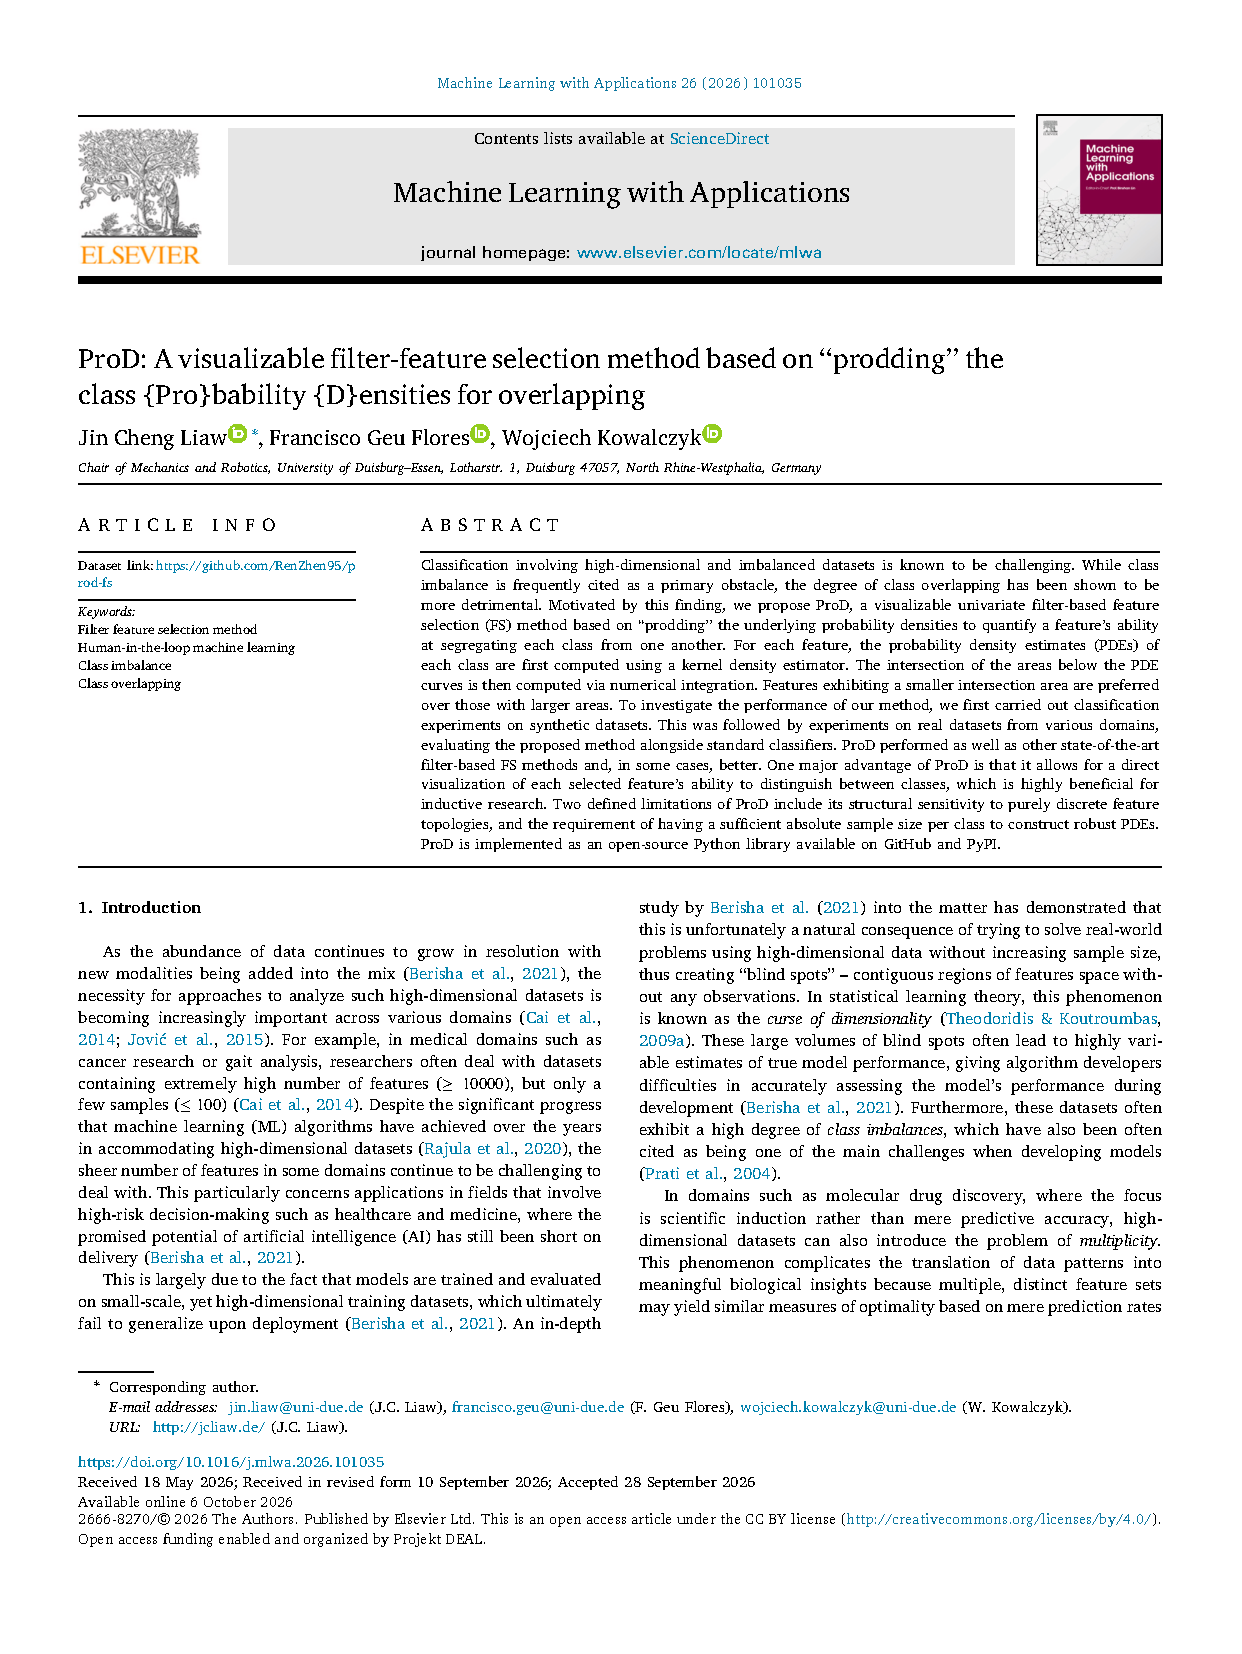
\includegraphics[height=5.0cm]{PaperScreenshot.pdf}
  \end{textblock*}
  
  %% QR Code
  \begin{textblock*}{2.2cm}(13.7cm, 2.65cm)
    \centering
    \begin{tabular}{r}
      {\tiny\color{udeBlue}\textbf{Read the paper}} \\ [-0.01cm]
      \qrcode[height=1.0cm]{https://doi.org/10.1016/j.mlwa.2026.101035}
    \end{tabular}
  \end{textblock*}
\end{frame}

% ==============================================================================
% OUTLINE
% ==============================================================================
\begin{frame}{Outline}
  \tableofcontents
\end{frame}

% ==============================================================================
% SECTION 1: MOTIVATION
% ==============================================================================
\section{Motivation}
\begin{frame}{Motivation}
  \begin{itemize}
  \item Classification involving \emph{high-dimensional} and \emph{imbalanced} datasets is challenging
  \item Often encountered in domains such as:
    \begin{itemize}
    \item Medicine \& Healthcare
    \item Genomic Research % Genomforschung
    \item Drug Discovery   % Arzneimittelforschung
    \end{itemize}
  \item Especially in applications involving high-risk decision-making, AI has still been short on delivery \cite{berisha2021}
  % Insbesondere bei Anwendungen, bei denen risikoreiche Entscheidungen getroffen werden müssen, hat die KI bislang noch nicht die Erwartungen erfüllt
  % Für eine ausführliche Behandlung des Themas kann ich das Paper hier empfehlen
    \begin{itemize}
    \item Curse of dimensionality: Few samples but high number of features \cite{berisha2021}
    \item High degree of class imbalances (?)
    \end{itemize}
  \item \textbf{Feature selection:}\\Reduce dimensionality by removing irrelevant and/or redundant features
  \end{itemize}

  \begin{textblock*}{2.2cm}(13.2cm, 5.75cm)
    \centering
    \begin{tabular}{r}
      {\tiny\color{udeBlue}\textbf{On challenges in}} \\ [-0.25cm]
      {\tiny\color{udeBlue}\textbf{high-risk applications:}} \\
      \qrcode[height=1.5cm]{https://doi.org/10.1038/s41746-021-00521-5}
    \end{tabular}
  \end{textblock*}
\end{frame}

\begin{frame}{Motivation -- Regarding Class Imbalance}
  \citet{prati2004} showed that very often class imbalance has been unfairly blamed for bad performance, when (quite) often \emph{class overlapping} is a larger culprit
  \begin{columns}[T]
    \begin{column}{0.52\textwidth}
      \hspace{0.05em} Take the original dummy example used in \cite{prati2004}:
      \begin{itemize}
      \item Positive priors vary (i.e. ``height'' of the distribution curve)
      \item Solid vertical line denotes optimal Bayes split
      \item Distributions are Gaussian and both have the same standard deviation (SD) but:
        \begin{itemize}
        \item (a) Means are 1 SD apart
        \item (b) Means are 4 SD apart
        \end{itemize}
      \end{itemize}
    \end{column}
    \begin{column}{0.48\textwidth}
      $\quad$ \\ [0.5cm]
      \footnotesize Solid -- Negative Class | Dotted -- Positive Class
      \\ [0.5cm]
      \resizebox{\linewidth}{!}{\input{PratiPicture.pdf_tex}}
    \end{column}
    \end{columns}
\end{frame}

\begin{frame}{Motivation -- Human-in-the-Loop Machine Learning}
  \begin{columns}[T]
    \begin{column}{0.52\textwidth}
      \begin{itemize}
      \item Pure data-driven techniques are inadequate (especially for high-risk decision-making) \cite{maadi2021}
        \begin{itemize}
          \item Quality highly depends on input data!
        \end{itemize}
      \item \textbf{Human-in-the-Loop Machine Learning:}\\Human experts intervene when models fail to generalize
        \begin{itemize}
        \item One key factor for this approach is \emph{transparency}
        \end{itemize}
      \end{itemize}
    \end{column}
    \begin{column}{0.48\textwidth}
    \end{column}
  \end{columns}
\end{frame}

\begin{frame}{Why Another Filter Feature-Selection Method?}
  \begin{columns}[T]
    \begin{column}{0.52\textwidth}
      \textbf{Limitations of Existing Approaches:}
      \begin{itemize}
        \item \textbf{Opaque Metrics:} Mutual Information (bits/nats) or ReliefF weights offer little geometric intuition.
        \item \textbf{Inductive Bias:} Hybrid methods (e.g., FeSNOC) couple feature ranking to downstream classifiers ($k$NN).
        \item \textbf{Memory Bottlenecks:} Instance-based filters scale at $\mathcal{O}(N^2)$ memory for distance matrices.
      \end{itemize}
    \end{column}
    \begin{column}{0.45\textwidth}
      \begin{block}{Core Idea of ProD}
        Evaluate each feature independently as a \textbf{pure filter} by directly measuring the geometric \textbf{Niche Overlapping Coefficient (NOC)} of its class-wise Kernel Density Estimates (KDE).
      \end{block}
      \vspace{0.3em}
      \begin{itemize}
        \item Bounded, intuitive score in $[0, 1]$
        \item Directly visualizable for human-in-the-loop diagnostics
      \end{itemize}
    \end{column}
  \end{columns}
\end{frame}


% ==============================================================================
% SECTION 2: METHODOLOGY
% ==============================================================================
\section{The ProD Methodology}

\begin{frame}{How ProD Measures Class Separability}
  \begin{columns}[c]
    \begin{column}{0.52\textwidth}
      \begin{enumerate}
        \item \textbf{Min-Max Normalization:} Scale feature $d$ to $[0, 1]$.
        \item \textbf{Class-Wise 1D KDE:} Estimate continuous probability density $\hat{p}_{d,c}(t)$ per class using Scott's rule.
        \item \textbf{Intersection Area (IA):} Compute geometric overlap across $k$-class combinations:
        \[
          A_{d, \mathcal{C}} = \int_0^1 \min_{c \in \mathcal{C}} \hat{p}_{d,c}(t) \, dt
        \]
        \item \textbf{Feature Ranking:} Rank features by ascending mean IA (less overlap $\Rightarrow$ higher separability).
      \end{enumerate}
    \end{column}
    \begin{column}{0.45\textwidth}
      \centering
      % Replace with your Figure 3 file (e.g., fig3_kde_overlap.pdf)
      \fbox{\parbox[c][4.8cm][c]{0.95\linewidth}{\centering
        \textbf{Insert Figure 3 Here}\\
        \scriptsize (3-Class KDE Overlap Plot showing $k=2$ vs. $k=|\mathcal{Y}|$)
      }}
    \end{column}
  \end{columns}
\end{frame}

%% % ==============================================================================
%% % SECTION 3: DIAGNOSTICS & MULTICLASS TUNING
%% % ==============================================================================
%% \section{Diagnostic Visualization \& Multiclass Tuning}

%% \begin{frame}{Uncovering Hidden Failure Modes with Pairwise Heatmaps}
%%   \begin{columns}[c]
%%     \begin{column}{0.50\textwidth}
%%       \textbf{The Pairwise Averaging Trap ($k=2$):}
%%       \begin{itemize}
%%         \item Averaging across all $\binom{|\mathcal{Y}|}{2}$ pairs can dilute localized failures.
%%         \item On the \textbf{HAR dataset}, top features cleanly separate \textit{Walking} vs. \textit{Laying}, but fail on \textit{Sitting} vs. \textit{Standing}.
%%       \end{itemize}
%%       \vspace{0.4em}
%%       \begin{block}{Solution: Higher-Order $k$}
%%         Setting $k = |\mathcal{Y}|$ penalizes localized cluster collapses, boosting HAR balanced accuracy from \textbf{0.631 to 0.828} (NN) and \textbf{0.627 to 0.863} (SVM).
%%       \end{block}
%%     \end{column}
%%     \begin{column}{0.47\textwidth}
%%       \centering
%%       % Replace with your Figure 11 file (e.g., fig11_har_heatmap.pdf)
%%       \fbox{\parbox[c][4.8cm][c]{0.95\linewidth}{\centering
%%         \textbf{Insert Figure 11 Here}\\
%%         \scriptsize (HAR Pairwise Intersection Area Heatmap)
%%       }}
%%     \end{column}
%%   \end{columns}
%% \end{frame}

%% % ==============================================================================
%% % SECTION 4: RESULTS & SOFTWARE
%% % ==============================================================================
%% \section{Experimental Validation \& Open-Source Tooling}

%% \begin{frame}{Key Results \& Complexity Guarantees}
%%   \begin{itemize}
%%     \item \textbf{Statistical Rigor (Friedman \& Nemenyi Tests):} Ranks \#1 in synthetic feature recovery (\textit{Suc.}) and is statistically rank-equivalent to top filters across real-world benchmarks.
%%     \item \textbf{Linear Space Complexity:} Scales at $\mathcal{O}(D \cdot |\mathcal{Y}| \cdot n_t)$, avoiding $\mathcal{O}(N^2)$ memory bottlenecks.
%%     \item \textbf{Built-In Safeguards:} Warns users when minority class size $N_c < 5$ (minimum required for stable IQR bandwidth estimation).
%%   \end{itemize}
%%   \vspace{0.5em}
%%   \begin{block}{Open-Source Python Package: \texttt{prod-fs} (v1.1.2)}
%%     \centering
%%     \texttt{pip install prod-fs} \quad $\bullet$ \quad Parallelized KDE + Built-in Distribution \& Heatmap Plots
%%   \end{block}
%% \end{frame}

%% % ==============================================================================
%% % THANK YOU / Q&A
%% % ==============================================================================
%% \begin{frame}[plain]
%%   \centering
%%   \insertUdeLogo{1.1cm}
%%   \vspace{1.2em}
  
%%   {\Large\bfseries\color{udeBlue} Thank You for Your Attention!}
%%   \vspace{1em}
  
%%   \begin{tabular}{rl}
%%     \textbf{Paper:} & \url{https://doi.org/10.1016/j.mlwa.2026.101035} \\
%%     \textbf{Package:} & \texttt{pip install prod-fs} \\
%%     \textbf{Contact:} & \textit{jin.liaw@uni-due.de} (University of Duisburg-Essen)
%%   \end{tabular}
%% \end{frame}

\begin{frame}[allowframebreaks]{References}
  \footnotesize
  \bibliography{references}
\end{frame}

\end{document}
